\def\pgfsysdriver{pgfsys-dvisvgm.def}
\documentclass[dvisvgm,tikz,border=8pt]{standalone}
\usepackage[compat=1.1.0]{tikz-feynman}

\begin{document}
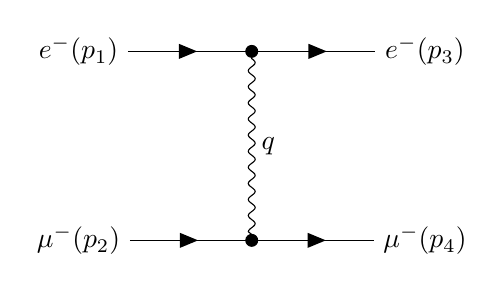
\begin{tikzpicture}
  \begin{feynman}
    \vertex (electron-in) at (-2.2,1.2) {$e^-(p_1)$};
    \vertex[dot] (electron-vertex) at (0,1.2) {};
    \vertex (electron-out) at (2.2,1.2) {$e^-(p_3)$};
    \vertex (muon-in) at (-2.2,-1.2) {$\mu^-(p_2)$};
    \vertex[dot] (muon-vertex) at (0,-1.2) {};
    \vertex (muon-out) at (2.2,-1.2) {$\mu^-(p_4)$};

    \diagram* {
      (electron-in) -- [fermion] (electron-vertex) -- [fermion] (electron-out),
      (muon-in) -- [fermion] (muon-vertex) -- [fermion] (muon-out),
      (electron-vertex) -- [photon, edge label={$q$}] (muon-vertex),
    };
  \end{feynman}
\end{tikzpicture}
\end{document}
